\section*{Exercise 1}
In this assignment, we implement the Random Projection Algorithm for reducing the number of dimensions in the MNIST dataset. 
The idea of random projections is simply if we have points in a vector space that are of sufficiently high dimension, then these points can be projected into a suitable lower-dimensional space in a way which approximately preserves the distances between the points.
we achieved this by randomly generate a k × d matrix with the assignment stated coefficients.
\begin{lstlisting}[frame=single]
def create_matrix(d, k)    
    mtx_val = 1/sqrt(d)
    prob = 0
    mtx = np.zeros((d, k))
    for i in range(0,d):
        for j in range(0,k):
            random_number = np.random.random_sample()
            if random_number <= 0.5:
                mtx[i,j] = mtx_val
            else:
                mtx[i,j] = -mtx_val        
    return mtx
\end{lstlisting}
    
Then we evaluate how well the Euclidean distance is preserved for the first 20 instances of the dataset by plotting the distortion for all the pairs.

Before plotting the distortion we expected its values to be between 0 and 1 (as proved in exercise 2) and also the value of distortion should approaches 1 when k increases because it will keep approaching the original d dimensions and thus less distortion.
   
Our expectations were confirmed by our experiment as in the below figures. 

In figure \ref{k50}, we can see that the most frequent value of distortion values is around 0.25 when k is 50
\begin{figure}[!htb]
\centering
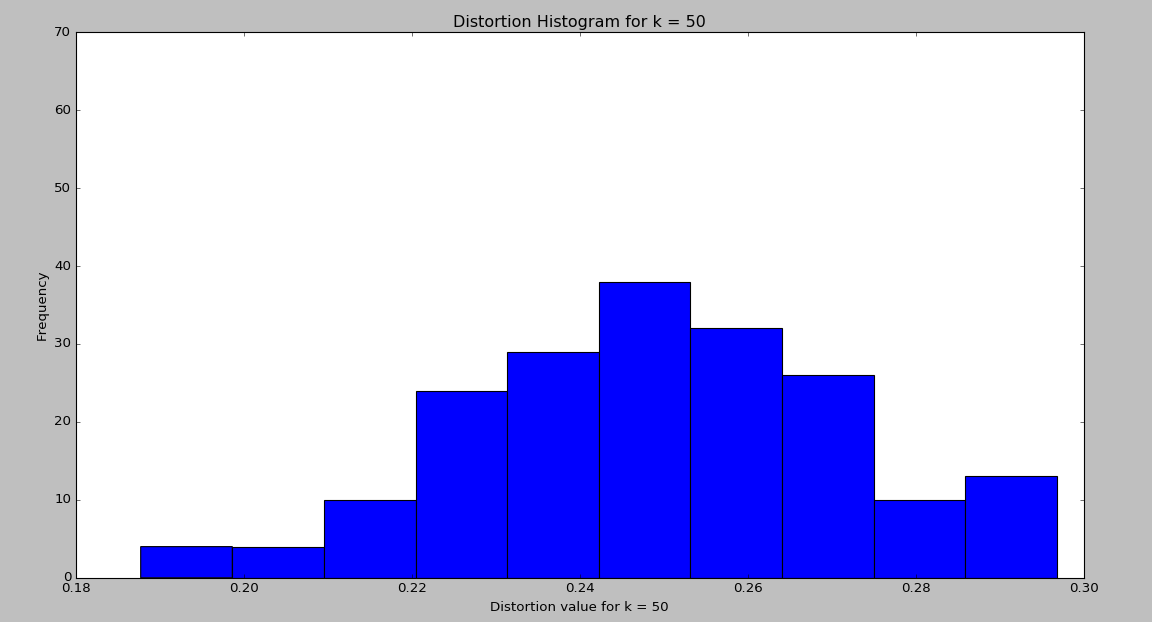
\includegraphics[width=0.9\textwidth]{shots/k50.png}
\caption{Histogram of the distortion values with k = 50  }
\label{k50}
\end{figure}

In figure \ref{k100}, the most frequent value of distortion values when k is 100 is around 0.35.

\begin{figure}[!htb]
\centering
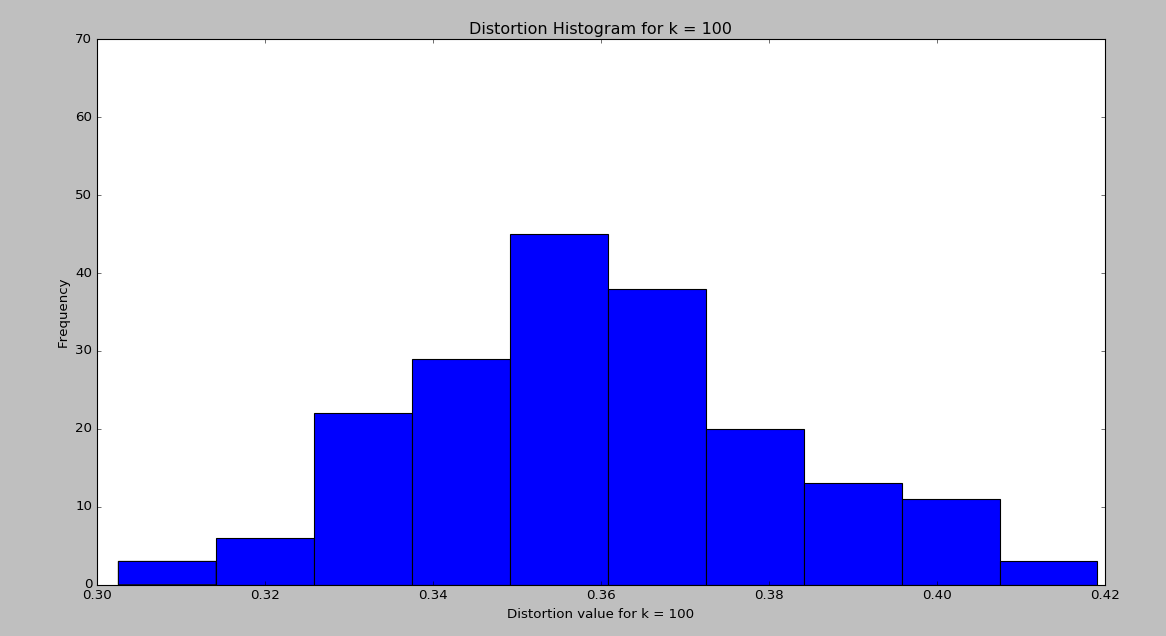
\includegraphics[width=0.9\textwidth]{shots/k100.png}
\caption{Histogram of the distortion values with k = 100 }
\label{k100}
\end{figure}

As we predicted, we can see that the distortion value increased to 0.79 when k is 500 as in figure \ref{k500}

\begin{figure}[!htb]
\centering
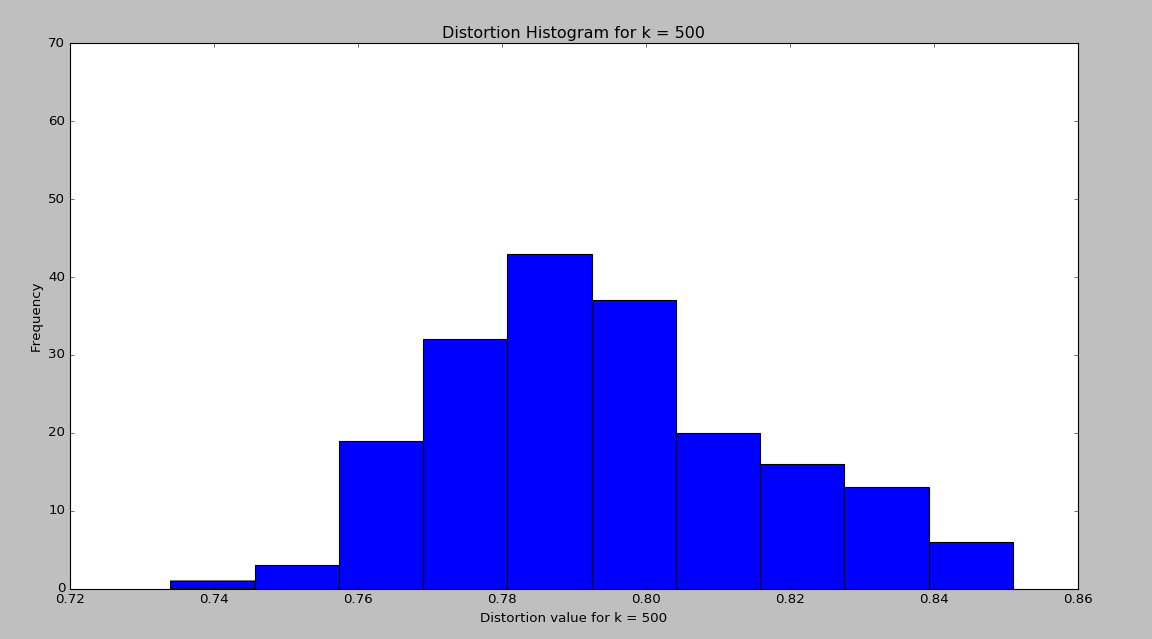
\includegraphics[width=0.9\textwidth]{shots/k500.png}
\caption{Histogram of the distortion values with k = 500 }
\label{k500}
\end{figure} 

In addition we changed our 1-NN implementation of Assignment 1a so that it uses the Euclidean distance instead of the cosine similarity as in the below function 

\begin{lstlisting}[frame=single]
def euclidean_distance(v1, v2):
    diff = np.subtract(v1, v2)
    return np.linalg.norm(diff)
\end{lstlisting}


We Run your implementation with and without random projection. But we scaled our vectors after the projection step to partially compensate for the distortion using a scaling factor $ \frac{\sqrt{d}}{\sqrt{k}} $ . Note that we run the implementation for 1000 test cases, as it takes a lot of time for 10,000 test cases we are running this 4 times to compare the results.

We measured the performance of 1-NN and we compared with and without random projection.
and we got the following results:

For 1-NN without Random Projections:

\begin{lstlisting}[frame=single]
Accuracy of the NN classifier is :  95.57 %

Class  0 :
Precision: 0.965517241379
Recall: 0.988235294118

Class  1 :
Precision: 0.9765625
Recall: 0.992063492063

Class  2 :
Precision: 0.982142857143
Recall: 0.948275862069

Class  3 :
Precision: 0.934579439252
Recall: 0.934579439252

Class  4 :
Precision: 0.962962962963
Recall: 0.945454545455

Class  5 :
Precision: 0.923076923077
Recall: 0.965517241379

Class  6 :
Precision: 1.0
Recall: 0.977011494253

Class  7 :
Precision: 0.920792079208
Recall: 0.939393939394

Class  8 :
Precision: 0.97619047619
Recall: 0.921348314607

Class  9 :
Precision: 0.927835051546
Recall: 0.957446808511
\end{lstlisting}

For 1-NN with Random Projections of K=50


\begin{lstlisting}[frame=single]
Accuracy of the NN classifier is :  92.3 %

Class  0 :
Precision: 0.955056179775
Recall: 1.0

Class  1 :
Precision: 0.932835820896
Recall: 0.992063492063

Class  2 :
Precision: 0.951923076923
Recall: 0.853448275862

Class  3 :
Precision: 0.92380952381
Recall: 0.906542056075

Class  4 :
Precision: 0.960784313725
Recall: 0.890909090909

Class  5 :
Precision: 0.873684210526
Recall: 0.954022988506

Class  6 :
Precision: 0.965517241379
Recall: 0.965517241379

Class  7 :
Precision: 0.92
Recall: 0.929292929293

Class  8 :
Precision: 0.890243902439
Recall: 0.820224719101

Class  9 :
Precision: 0.852941176471
Recall: 0.925531914894

\end{lstlisting}

For 1-NN with Random Projections of K=100



\begin{lstlisting}[frame=single]
Accuracy of the NN classifier is :  94.0 %

Class  0 :
Precision: 0.976744186047
Recall: 0.988235294118

Class  1 :
Precision: 0.9765625
Recall: 0.992063492063

Class  2 :
Precision: 0.972972972973
Recall: 0.931034482759

Class  3 :
Precision: 0.924528301887
Recall: 0.915887850467

Class  4 :
Precision: 0.960784313725
Recall: 0.890909090909

Class  5 :
Precision: 0.870967741935
Recall: 0.931034482759

Class  6 :
Precision: 0.965909090909
Recall: 0.977011494253

Class  7 :
Precision: 0.932038834951
Recall: 0.969696969697

Class  8 :
Precision: 0.95
Recall: 0.85393258427

Class  9 :
Precision: 0.864077669903
Recall: 0.946808510638
\end{lstlisting}


For 1-NN with Random Projections of K=500


\begin{lstlisting}[frame=single]
Accuracy of the NN classifier is :  95.6 %

Class  0 :
Precision: 0.943820224719
Recall: 0.988235294118

Class  1 :
Precision: 0.984251968504
Recall: 0.992063492063

Class  2 :
Precision: 0.981981981982
Recall: 0.939655172414

Class  3 :
Precision: 0.942857142857
Recall: 0.92523364486

Class  4 :
Precision: 0.963963963964
Recall: 0.972727272727

Class  5 :
Precision: 0.893617021277
Recall: 0.965517241379

Class  6 :
Precision: 0.977011494253
Recall: 0.977011494253

Class  7 :
Precision: 0.949494949495
Recall: 0.949494949495

Class  8 :
Precision: 0.963414634146
Recall: 0.887640449438

Class  9 :
Precision: 0.947368421053
Recall: 0.957446808511
\end{lstlisting}


we can see that the performance of the classifier with projections of K=50 and K=100 is lower than the performance without projections as this huge dimensionality reduction cause loss of information. but we can see the performance is improving with the increasing of K.
And for K=500, the performance became better than the classifier without projections and the cause could be some noise and outliers that their effect was reduced with our dimensionality reduction by random projections.  